% \begin{figure*}[t!]
%     \centering
%     % --- 第一张子图 ---
%     \begin{subfigure}[b]{0.48\textwidth}
%         \centering
%         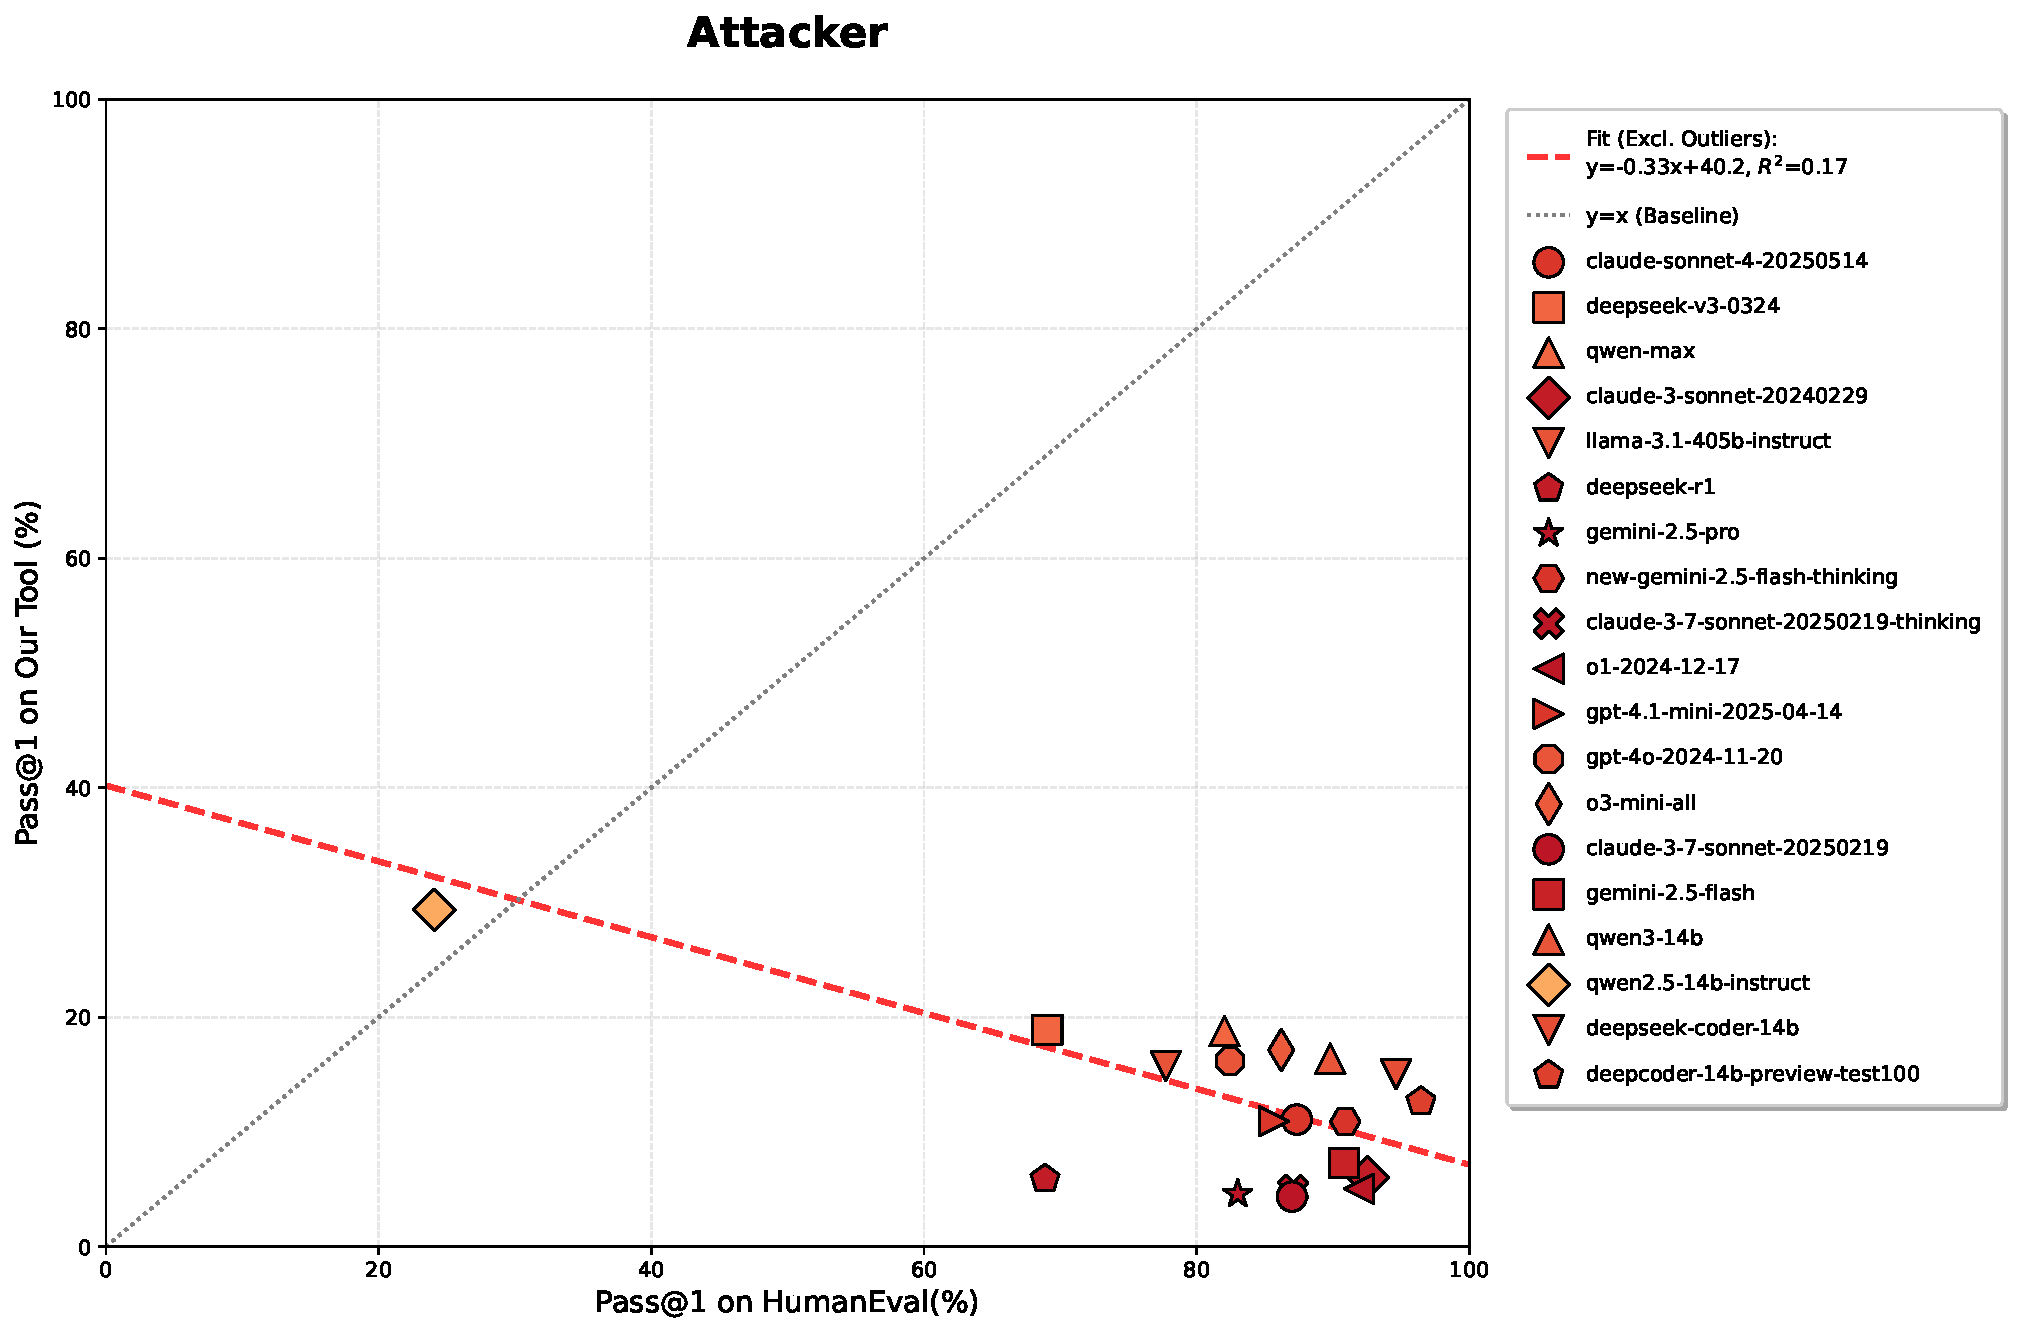
\includegraphics[width=\textwidth]{figures/attacker-weighted-fixed.pdf}
%         \caption{Attacker perspective}
%         \label{fig:exp2_def_attacker}
%     \end{subfigure}
%     \hfill
%     % --- 第二张子图 ---
%     \begin{subfigure}[b]{0.48\textwidth}
%         \centering
%         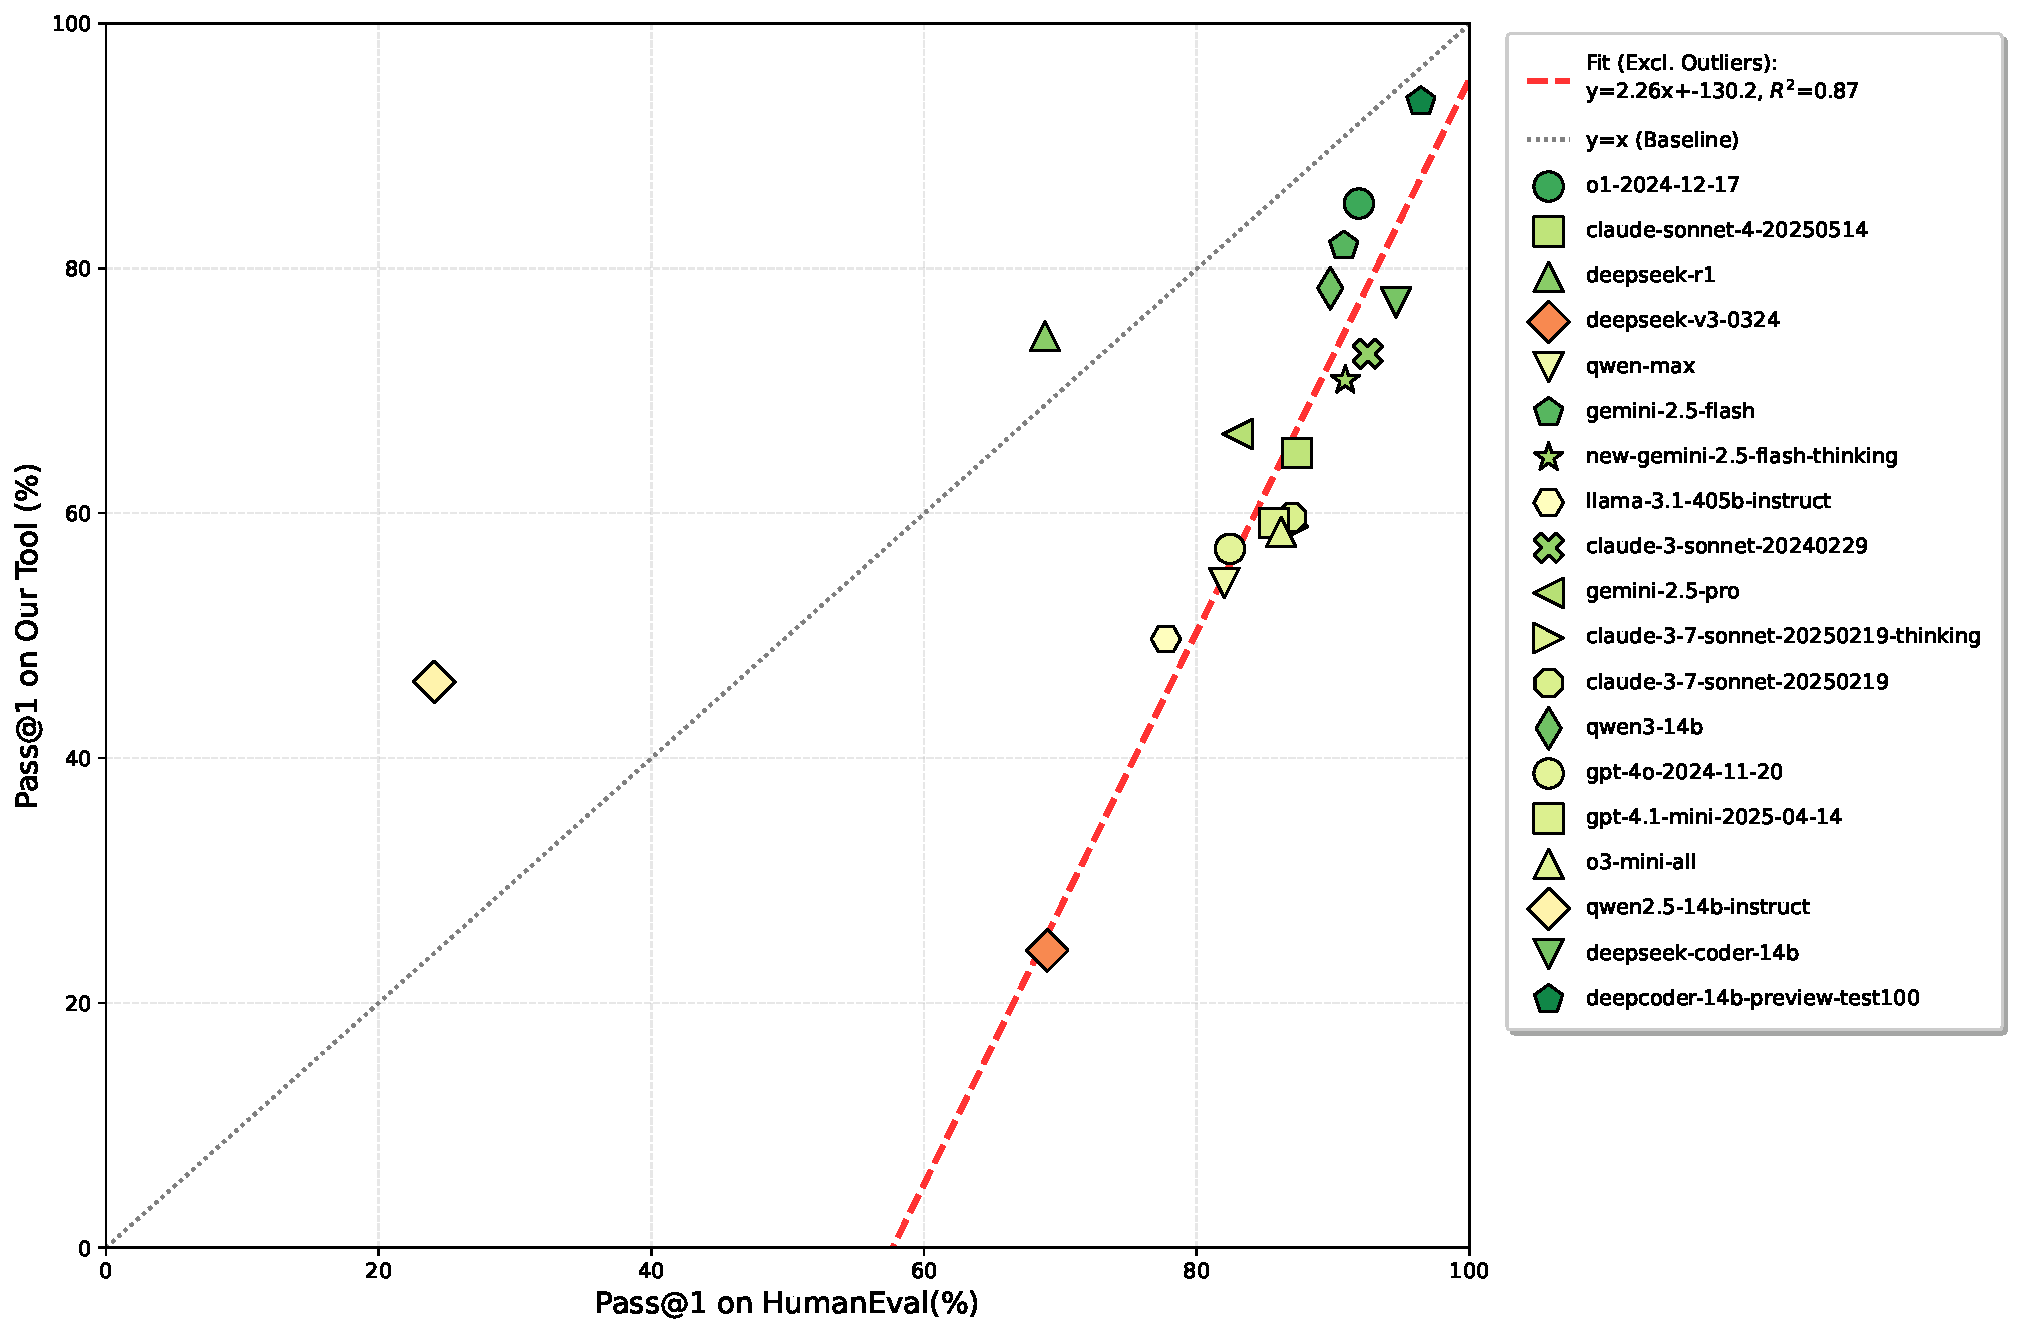
\includegraphics[width=\textwidth]{figures/defenderweightedfixed.pdf}
%         \caption{Defender perspective}
%         \label{fig:exp2_def_defender}
%     \end{subfigure}

%     \vspace{4mm}
%     \caption{\tool{} vs HumanEval: comparison from both perspectives. The results show the performance difference between attacker and defender workflows.}
%     \label{fig:exp2_def}
% \end{figure*}



\begin{figure}[!htbp]
  \captionsetup{skip=5pt}
  \centering
  
  \begin{subfigure}[b]{0.48\textwidth}
    \centering
    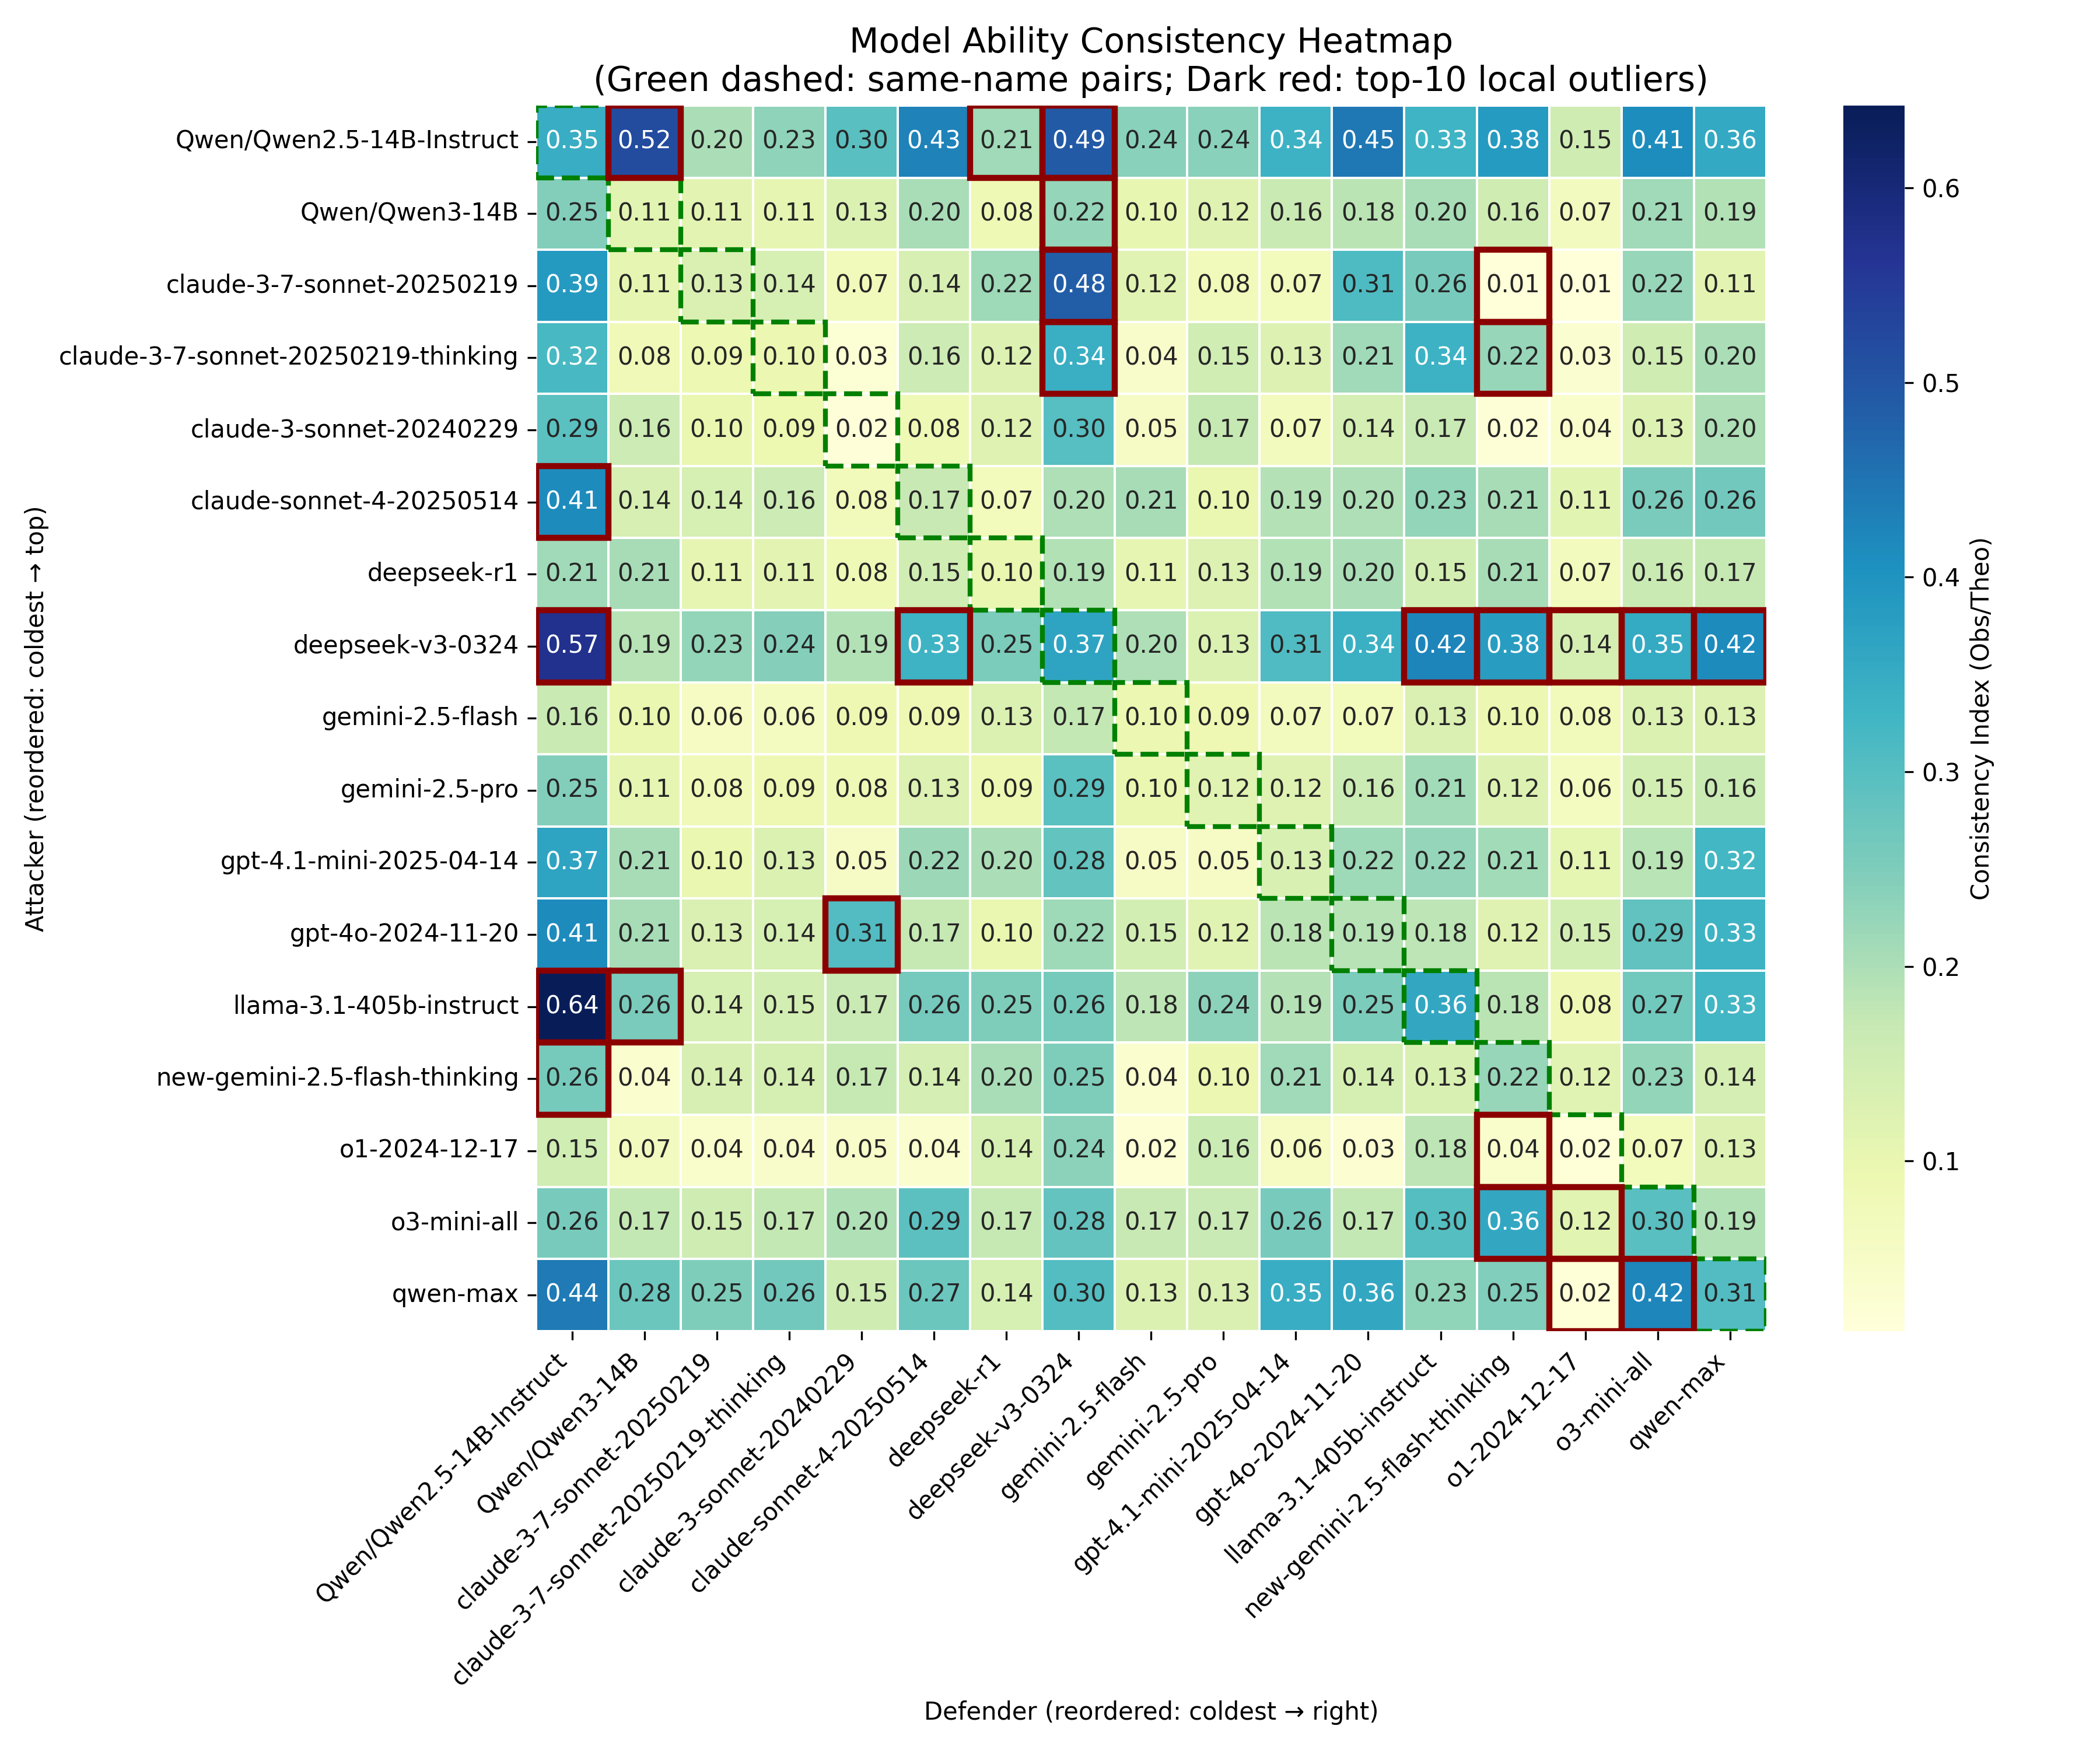
\includegraphics[width=\textwidth]{figures/styleconsistencyheatmaporiginal.png}
    \caption{Attacker workflow}
    \label{fig:figattattacker}
  \end{subfigure}
  \hfill
  \begin{subfigure}[b]{0.48\textwidth}
    \centering
    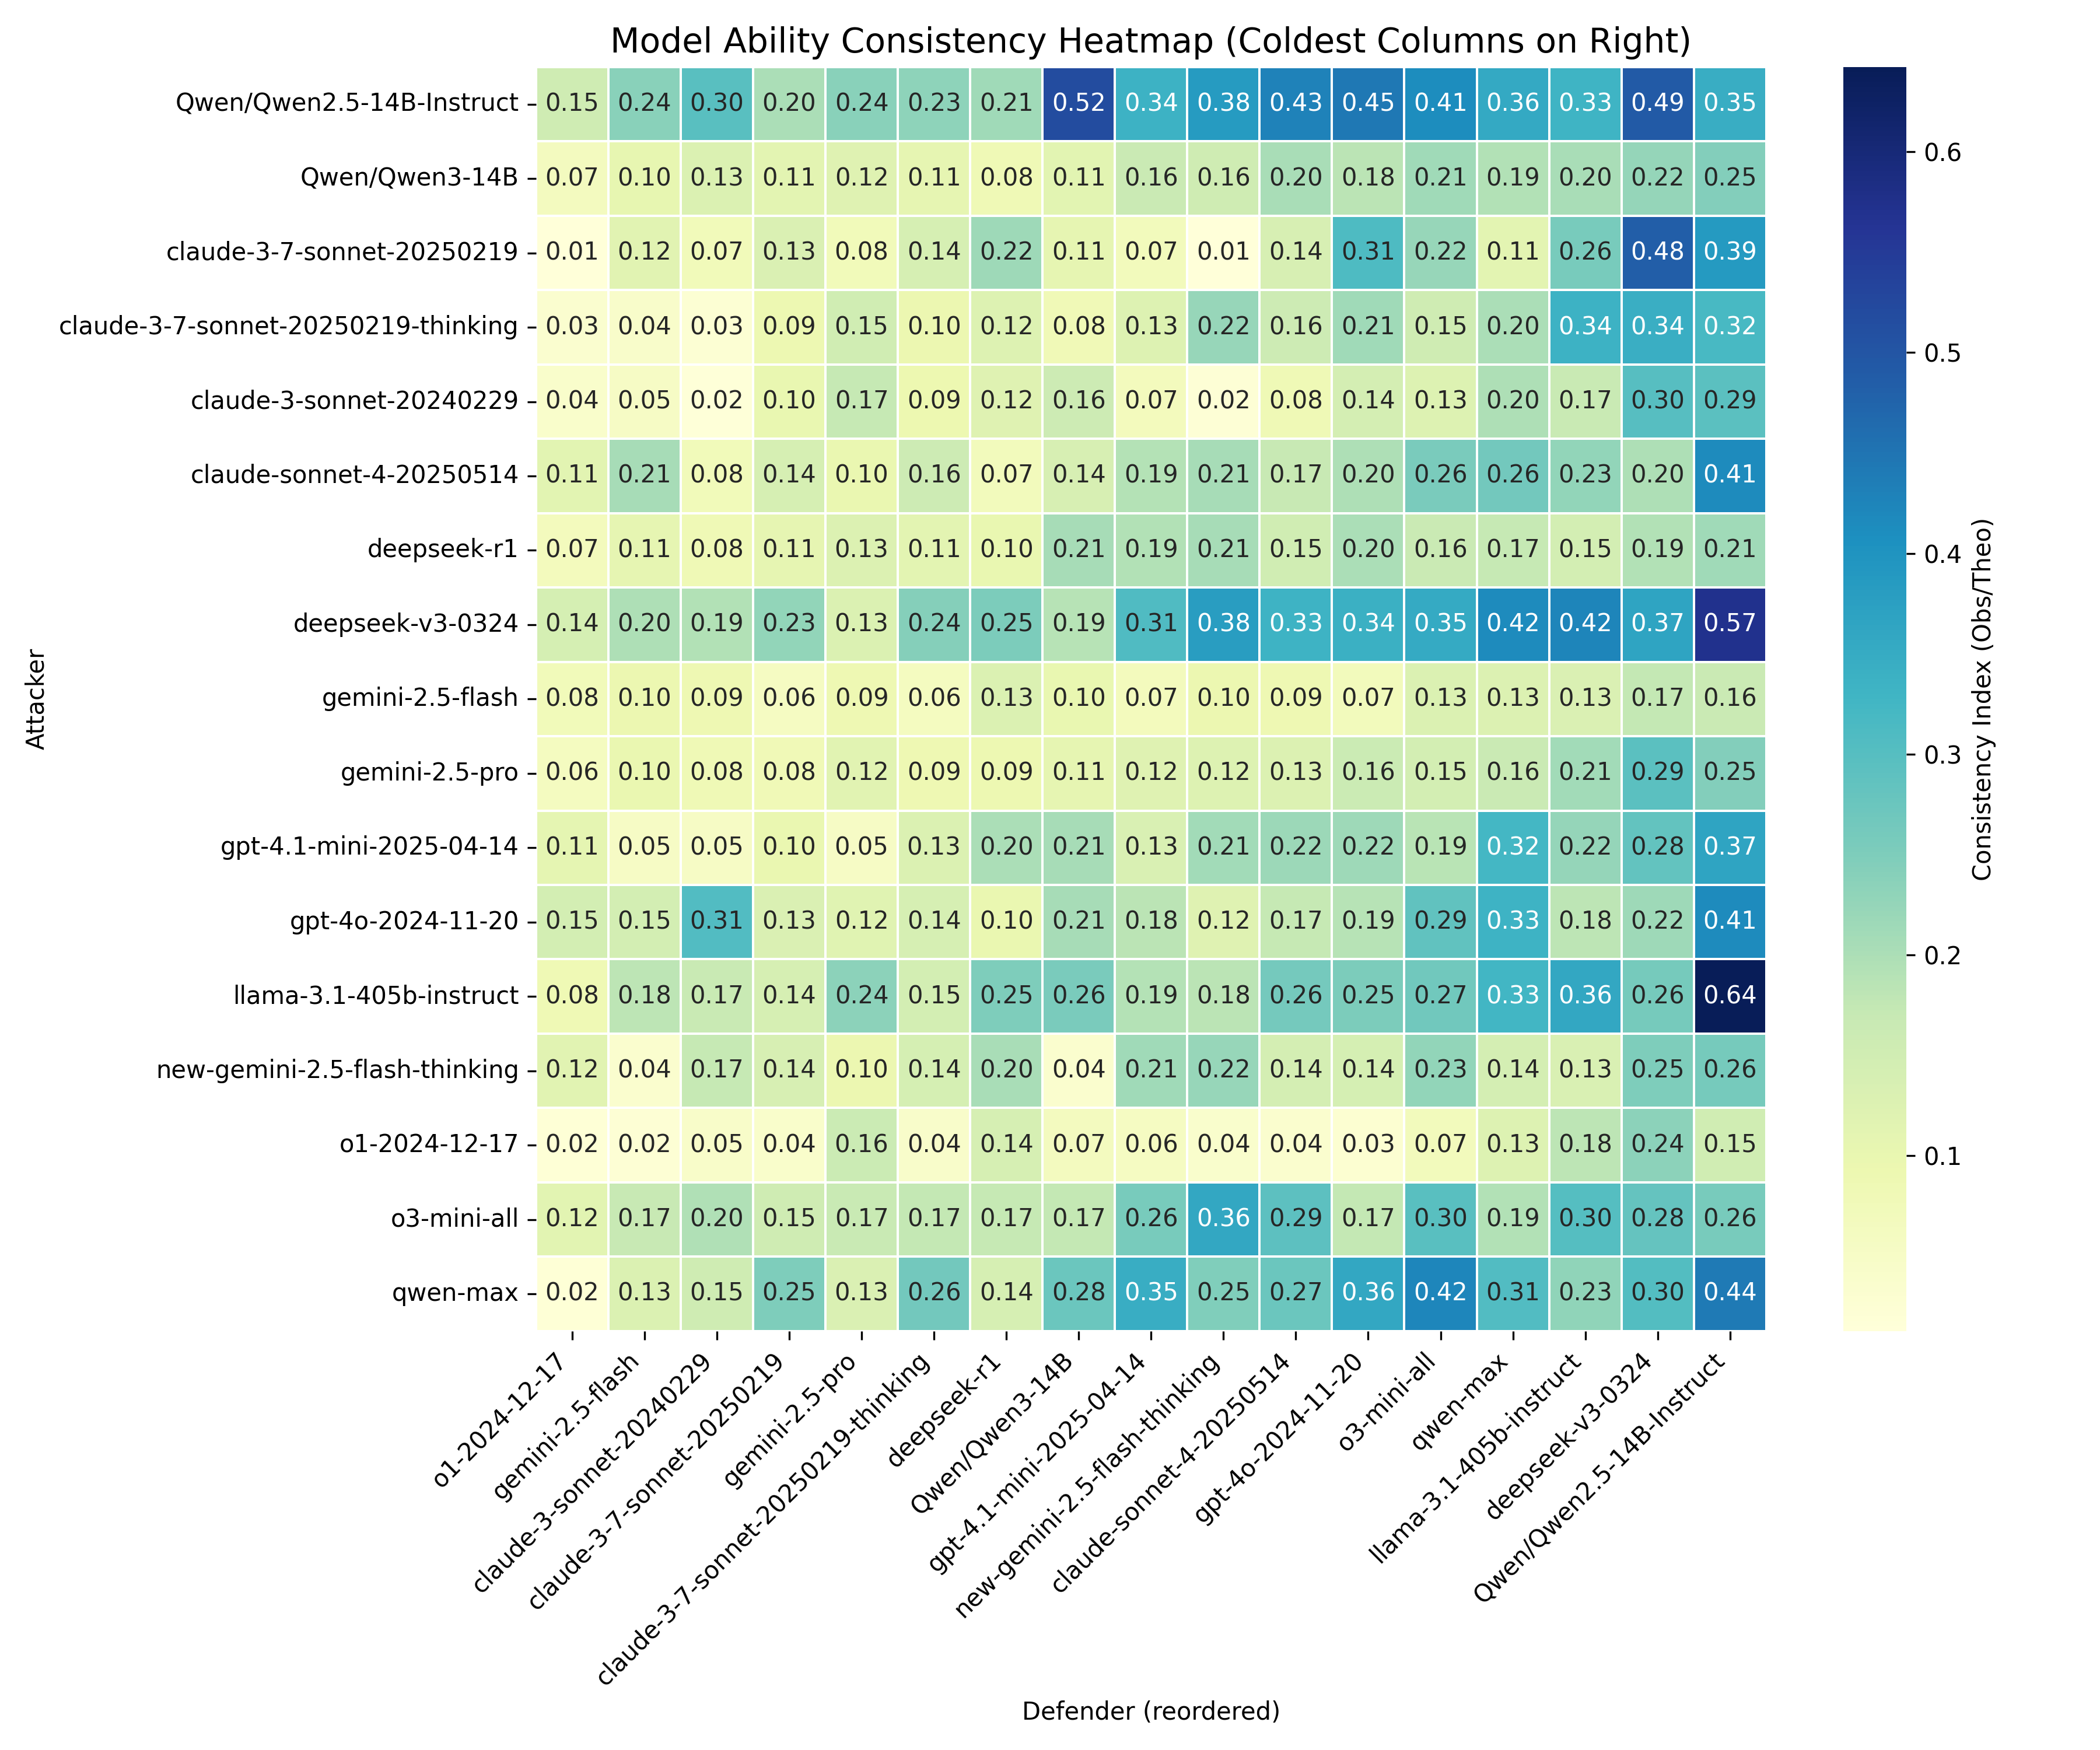
\includegraphics[width=\textwidth]{figures/styleconsistencyheatmap222.png}
    \caption{Defender workflow}
    \label{fig:figattdefender}
  \end{subfigure}
  
  \caption{\tool's workflow: attacker vs defender perspective}
  \Description{Two heatmaps comparing style consistency from the attacker perspective and the defender perspective.}
  \label{fig:figatt}
\end{figure}